\documentclass[11pt,a4j]{jarticle}
\usepackage[dvipdfmx]{graphicx,color}
\usepackage{wrapfig}
\setlength{\topmargin}{-1.5cm}
\setlength{\textwidth}{15.5cm}
\setlength{\textheight}{25.2cm}
\newlength{\minitwocolumn}
\setlength{\minitwocolumn}{0.5\textwidth}
\addtolength{\minitwocolumn}{-\columnsep}
%\addtolength{\baselineskip}{-0.1\baselineskip}
%
\def\Mmaru#1{{\ooalign{\hfil#1\/\hfil\crcr
\raise.167ex\hbox{\mathhexbox 20D}}}}
%
\begin{document}
\newcommand{\fat}[1]{\mbox{\boldmath $#1$}}
\newcommand{\D}{\partial}
\newcommand{\w}{\omega}
\newcommand{\ga}{\alpha}
\newcommand{\gb}{\beta}
\newcommand{\gx}{\xi}
\newcommand{\gz}{\zeta}
\newcommand{\vhat}[1]{\hat{\fat{#1}}}
\newcommand{\spc}{\vspace{0.7\baselineskip}}
\newcommand{\halfspc}{\vspace{0.3\baselineskip}}
\bibliographystyle{unsrt}
%\pagestyle{empty}
\newcommand{\twofig}[2]
 {
   \begin{figure}[h]
     \begin{minipage}[t]{\minitwocolumn}
         \begin{center}   #1
         \end{center}
     \end{minipage}
         \hspace{\columnsep}
     \begin{minipage}[t]{\minitwocolumn}
         \begin{center} #2
         \end{center}
     \end{minipage}
   \end{figure}
 }
%%%%%%%%%%%%%%%%%%%%%%%%%%%%%%%%%
%\vspace*{\baselineskip}
\begin{center}
{\Large \bf 令和1年度 共同研究報告書}
\end{center}
\vspace{2mm}
\begin{center}
{\LARGE \bf 結晶質岩を対象とした連成現象が\\
長期挙動におよぼす影響に関する研究} 
\end{center}
\begin{center}
岡山大学環境生命科学研究科\\
木本和志, 市川康明
\end{center}
\vspace{10mm}
%%%%%%%%%%%%%%%%%%%%%%%%%%%%%%%%%%%%%%%%%%%%%%%%%%%%%%%%%%%%%%%%
\section{はじめに}
結晶質岩中のマイクロクラックは、岩盤の長期的な物質輸送特性や力学的な挙動に影響を与えると
考えられる。マイクロクラックの多くは肉眼で直接観測することは難しく、薄片を作成し偏光顕微鏡で
観察するなどして調べる必要がある。このような検査は非常に労力を要する上、
検査対象となる岩の状態をその場で非破壊的に調べる際には利用できない。
そのため、その場かつ非破壊的にマイクロクラックの状態を調べる技術があれば、
岩盤の現在の状態や長期の将来的な挙動を予想する上で有用な情報を提供刷ることができる。
そのような観点のもと、著者らは、超音波を使った花崗岩コア供試体の音響的性質の評価に
取り組んで来た。その結果としてこれまでに、粗大な結晶粒を有する花崗岩であっても、
数cm程度の距離であれば、数mmスケールの超音波を透過させることができることを示した。
また、レーザードップラー振動計を用いて波動場を詳細に観測することで、
鉱物粒と弾性波の相互作用を可視化できること、試料の部位や状態に応じて表面波速度に
有意な変化が現れることも明らかにしてきた。
これら音速の変化は、波動場の可視化結果からマイクロクラックの状態を
反映したものと予想されるものの、き裂の存在によって岩石の音響的性質が変化することの
より確実な証拠を見出すことが課題として残されていた。
花崗岩では、造岩鉱物自体が異方性を持ち、き裂が存在せずとも、異方性や散乱による
弾性波の減衰が起きる。そのため、みかけの異方性や減衰が観測されることから、
き裂の影響であるとそのまま結論を導くことはできない。
一方で、き裂は、岩盤が受ける応力場に起因して発生や進展した場合、応力場に応じた
配向性を示すことや、特定の鉱物に集中して発生する可能性が予想される。
従って、き裂の発生や成長に伴う音響異方性の変化や、特定の鉱物種の周辺で
生じる特異な散乱、鉱物種の含有割合におうじた音響的性質の変化を観察することが
き裂と弾性波の相互作用を理解し、計測波形からき裂の状態を推定する上で必要となる。
そのためには、鉱物粒からコアサンプルのスケールまで種々の空間解像度で弾性波散乱や
音響異方性を調べる方法が必要となる。
従来、岩石コアの音響的性質の評価では、圧電トランスデューサでコアサンプルを
透過した波動を計測しその音速や異方性を調べることが行われてきた。
この方法では、コア全体の平均的な性質は調べることができるものの、コアの部位や
鉱物の分布状況に応じてた音響的な性質の評価は行うことができない。
また、超音波を透過させることのできる方向は供試体の形状によって決まるため、
状況によっては、透過波を計測ができない方向もあり、音響異方性を調べることができない
場合もある。このことから、クラックの状態を知るための弾性波計測は、
供試体表面の任意の位置と方向で実施可能な方法を用いることが望ましい。
本年度の研究では、そのような計測の実現に向け、同一表面において、任意の方向と伝播
距離で超音波の送信と受信と行う方法を提案し、音響異方性の評価に利用可能である
ことを示した。具体的には、コアサンプル中央の
20mm角の領域が示す音響異方性を超音波波形から推定し、マイクロクラックに起因した
直交異方性が観察できることを明らかにする。
以下では、新たに構築した超音波計測系と 実験に用いた花崗岩コア供試体について述べる。
特に、強い超音波を送信するために新たに導入した集束型接触探触子の仕様と
導入の意図を述べる。計測点の配置や波形収録に関する設定について示した後、
実際に構築した計測系で得た超音波波形を示す。
次に、超音波波形から岩石コア試料の音響的性質を得るために、行った
波形処理の方法とその結果得られた音速やピーク周波数を示す。
最後に、入射方向によるそれら音響的性質の変化を示し。花崗岩よく知られている通り、
直交異方性を示すことが、表面波計測結果からも示されること、さらに、
波形振幅と音速の相関から、異方性はき裂に起因したものであることが示唆されることを
述べ、まとめと今後の課題について述べる。

\section{超音波計測実験の方法}
花崗岩コアを伝播する弾性波を計測するため行った実験の方法について述べる。
以下でははじめに、実験に用いたコアサンプルについて、次に、強い弾性波を励起する
ために設計、制作した圧電超音波トランスデューサについて述べた後,計測システム全体の構成
と計測点の配置を示す。
\subsection{実験供試体}
超音波計測に用いた花崗岩供試体の外観と、形状および大きさを図\ref{fig:fig1}に示す。
供試体は、岡山県万成の採石場で採取した万成花崗岩を円柱状に加工したもので、直径は
約66mm, 高さは60mmである。主要造岩鉱物は石英、雲母、ナトリウムおよびカリ長石で。
数mmから数cm程度の結晶粒から構成される。外観からは肉眼で観察できるき裂などはなく、
風化もや造岩鉱物の明らかな変質も認められない。
ここで、供試体内部と表面の位置を指定するための$XYZ$直交座標を図\ref{fig:fig1}の
(b)および(c)のように取る。超音波の送信と受信は、供試体の上面$(Z=0)mm$で行い,
主として直径方向に伝播する表面波を観測する。
%--------------------
\begin{figure}[h]
	\begin{center}
	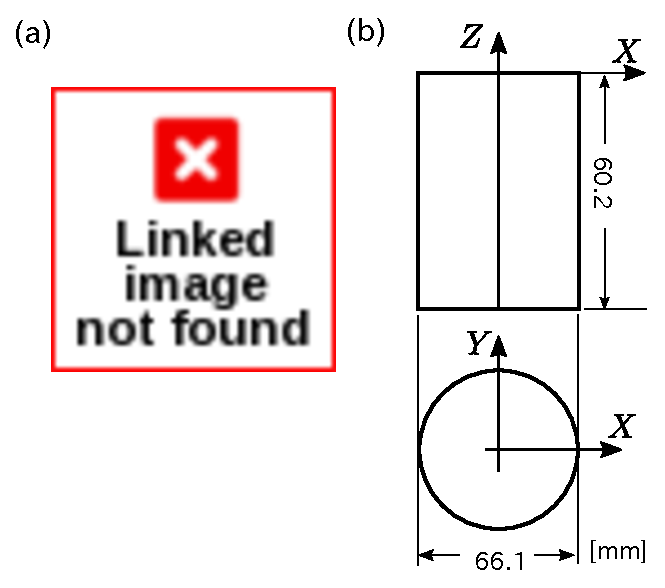
\includegraphics[width=0.6\linewidth]{Figs/fig1.eps} 
	\end{center}
	\caption{
		超音波計測に用いた花崗岩コア供試体(万成花崗岩).
	} 
	\label{fig:fig1}
\end{figure}
%--------------------
\subsection{超音波トランスデューサ}
本年度の実験のために、超音波を送信するための接触型ラインフォーカス・トランスデューサを設計、制作した。
圧電超音波トランスデューサの構成を図\ref{fig:fig2}に示す。
曲率をもった圧電素子がくさび状のポリエーテルイミドのシューにマウントされている。
圧電素子の曲率中心はシューの先端部にある。
シュー先端部の幅は1mmで、圧電素子の周波数は2MHz.
花崗岩試料の弾性波速度は、縦波が約5km/s, 横波が3km/s程度であることがわかっている。
そのため、2MHzの超音波の岩石試料内部での波長は縦波。横波のそれぞれ、およそ2.5mm, 1.5mm程度となる。
試料表面の方向に十分な強度の超音波を送信するためには、シュー先端の幅は波長程度の寸法にする必要がある。
ここでは、先端部の幅を2MHzの横波波長よりも小さくなるよう、1mmとした。
圧電素子の幅は、シュー先端部の幅と岩石中での超音波の波長よりも十分に長くなるよう
40mmとした。これにより、線音源に近い状態を作り、平面波を励起する。
完全な平面波は距離による減衰が無く、伝播挙動を理解しやすい。
このことは、岩石のような強い散乱減衰を起こす、不均質材中の弾性波挙動を調べる上で重要である。
%--------------------
\begin{figure}[h]
	\begin{center}
	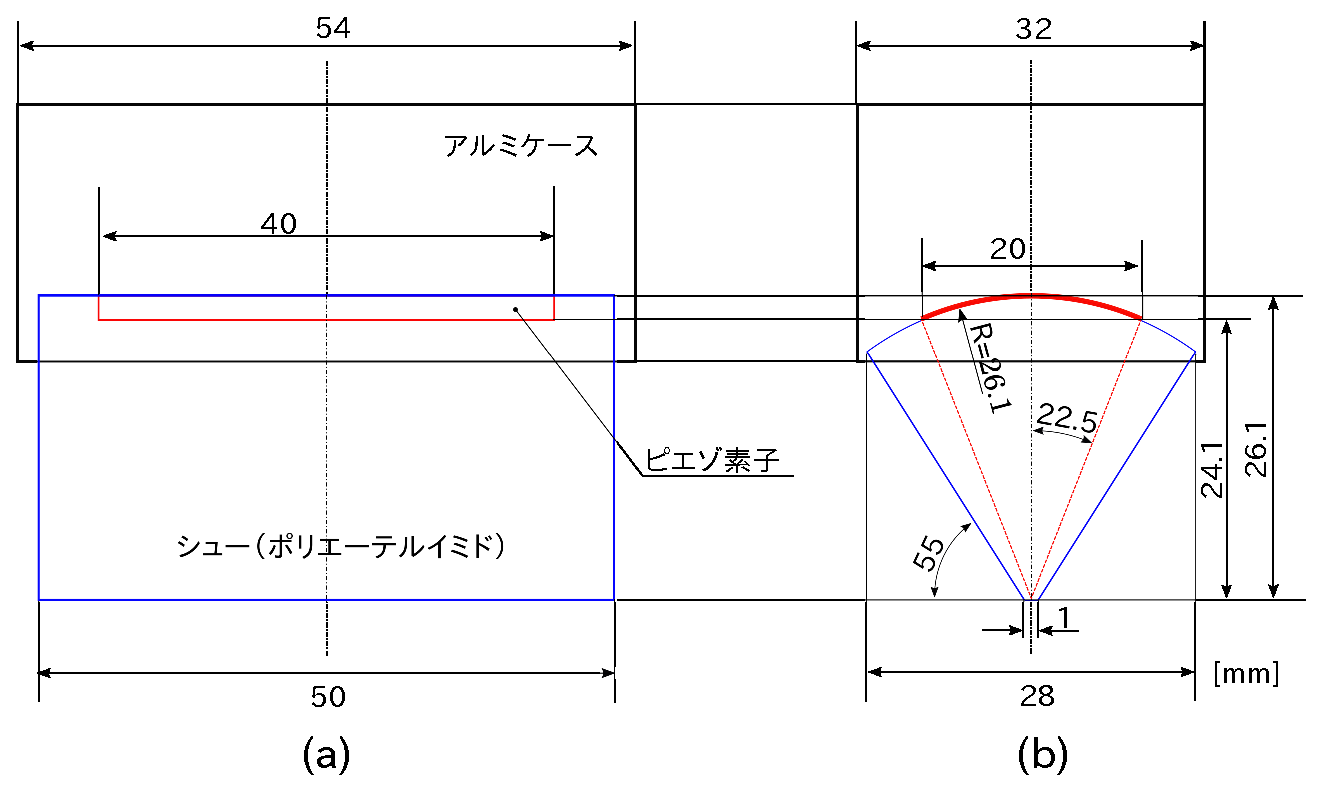
\includegraphics[width=0.8\linewidth]{Figs/fig2.eps} 
	\end{center}
	\caption{
		接触型ラインフォーカス探触子の形状と寸法.
	} 
	\label{fig:fig2}
\end{figure}
%--------------------
\subsection{超音波計測系の構成}
超音波計測システムの構成を図\ref{fig:fig3}に示す。
花崗岩コア試料は、3軸ステージ上に固定する。
3軸ステージは、平面内xy方向へ並進2軸、鉛直方向を回転軸とする回転1軸を持つ。
各ステージはステッピングモーターで駆動され、試料の位置と向きを正確に調整するために用いる。
送信に用いるラインフォーカストランスデューサは、コア供試体上面に接触させて固定する。
受信には、レーザードップラー振動計(LDV: laser Doppler vibrometer)を用いる。
LDVは、高い空間解像度と十分な周波数帯域を持つことから、ここでの計測に理想的なものである。
ただし、試料表面の状態により信号−雑音比(SN比)が大きく変化することが問題となる。
ここでは十分な反射レーザー光の受光感度を得るため、
コア供試体の上面にアルミ箔を貼り付けている。
アルミ箔は、供試体表面にオイルを均等に塗り、供試体とアルミ箔の間に空隙を残さないように貼り付けている。
送信に用いるトランスデューサは、超音波探傷試験用のパルサーレシーバから、矩形パルスを
印加して励起する。LDVは、LDVコントローラを介して制御PCとオシロスコープに接続する。
オシロスコープでは、LDVで計測した速度波形の取り込みを、パルサーレシーバと同期して行う。
一方、制御PCは、LDVコントローラ、オシロスコープとシリアル通信を行う。
PCとはLDVから受光感度のデータを受け取り、計測点毎にフォーカス調整機能を動作させる。
オシロスコープからはLDVから取り込みデジタイズされた波形を取得する。
また、制御PCは3軸ステージの移動をステージコントローラを介して行う。
以上、LDVのフォーカス調整、受光感度記録、波形取り込み,ステージ制御による計測点位置調整を、
本システムでは、PCからのシリアル通信によるコマンド制御で行うことで、一連の計測を自動化して行うことができる。
%--------------------
\begin{figure}[h]
	\begin{center}
	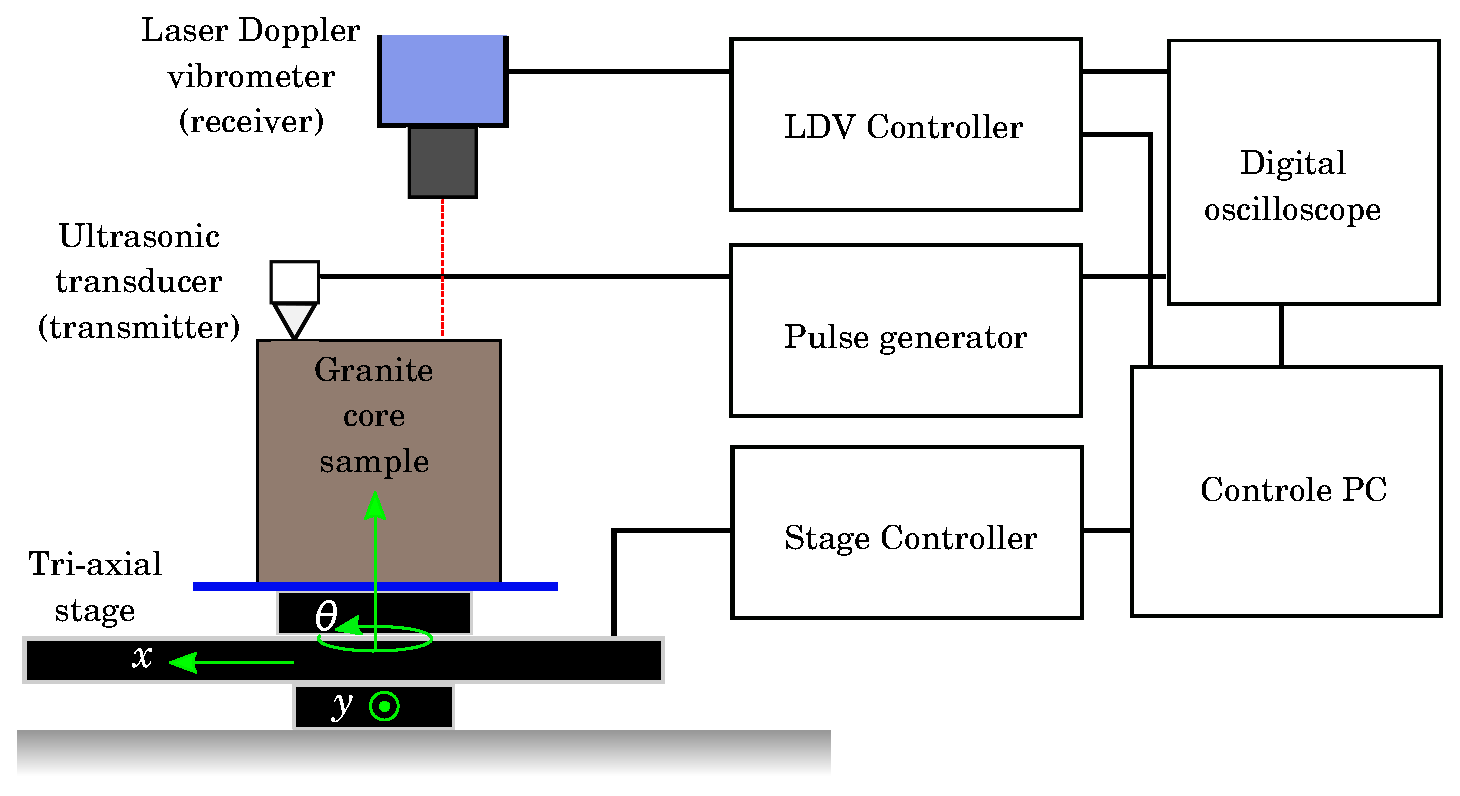
\includegraphics[width=0.8\linewidth]{Figs/fig3.eps} 
	\end{center}
	\caption{
		超音波測定装置の構成.
	} 
	\label{fig:fig3}
\end{figure}
%--------------------
\subsection{送受信点の配置}
超音波の送受信点位置を指定するために、図\ref{fig:fig4}に示すような
$xy$座標系を、供試体上面($Z=0$)にとる。$xy$座標は、$XY$座標と反時計回りの方向に
$\theta$だけ向きが異なるものとする。
ここで、$x$軸は、入射波の伝播方向を向くようにとることとする。
すなわち、X軸から測った角度$\theta$で入射波の伝播方向を表す。
$\theta$方向に超音波を入射するために、ラインフォーカストランスデューサは、
図\ref{fig:fig4}の$\cal S$で示した位置にシュー先端部を接触させて固定する。
一方、LDVによる超音波の受信は,同図で${\cal R}$として示した測線上を0.5mmのピッチで
行う。測線の長さは20mmとしているため、測定点数は41点となる。
送信位置$\cal S$、受信位置$\cal R$はは、いずれも
コア供試体の中心($(x,y)=(0,0)$mmから20mm離れた位置とし、これにより、40mmの距離
を伝播した超音波の上下動($Z$方向成分)を計測する。
このような計測を入射角$\theta$を0度から330度まで30度ピッチで行い、計12の入射
方向について供試体の直径方向に伝播する超音波の計測を行う。
\begin{enumerate}
\item パルサー設定
	\begin{itemize}
		\item 電圧パルス形状:矩形
		\item 印加電圧: -400V
		\item パルス幅: 0.25$\mu$sec 
		\item パルス繰り返し周波数:2kHz
	\end{itemize}
\item 波形収録条件
	\begin{itemize}
		\item サンプリング周波数:40MHz
		\item サンプリング点数:4,000点
		\item 計測時間範囲:0$\sim$100$\mu$sec
		\item 平均化回数:4,096回
	\end{itemize}
\item 送受信点配置
	\begin{itemize}
		\item 入射方向$\theta$[deg]:
			\[
				\left\{ 
				\theta=k \Delta \theta \left| \Delta \theta=30,\, k=0,1,\dots 11\right.
				\right\}
			\]
		\item 送信位置[mm]:
			\[
				{\cal S}=\left\{ (x,y)\left| x=-20, |y| \leq 20\right.\right\}, \ \ 
			\]
		\item 受信位置[mm]:
			\[
				{\cal R}=\left\{ (x,y)\left| x=20,  |y| \leq 10\right.\right\}, \ \ 
			\](0.5mmピッチ)
		\item 透過距離:$L$=40mm
	\end{itemize}
\end{enumerate}
%--------------------
\begin{figure}[h]
	\begin{center}
	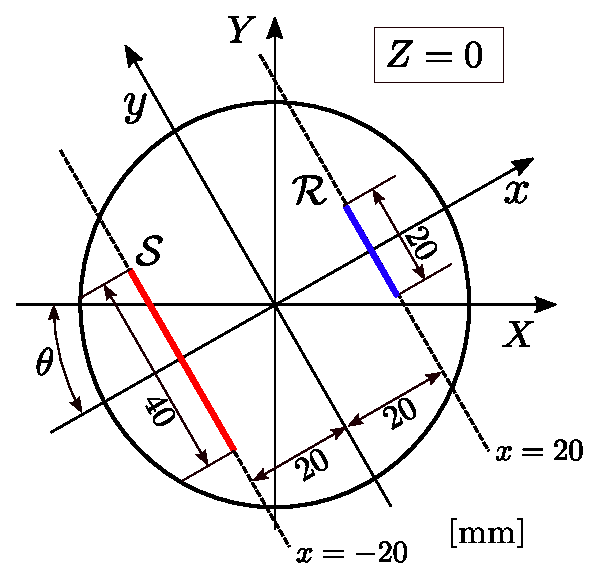
\includegraphics[width=0.5\linewidth]{Figs/fig4.eps} 
	\end{center}
	\caption{
		花崗岩コア供試体の上面における超音波送受信位置の配置.
		${\cal S}$は,ラインフォーカス探触子のカップリング位置を,
		${\cal R}$は,レーザー振動計による計測の測線を表す.
	} 
	\label{fig:fig4}
\end{figure}
%--------------------


\section{超音波計測結果}
\subsection{送信波形の計測}
ラインフォーカス探触子先端部を供試体に接触させず、自由に振動させたときの挙動を調べた。
振動波形の取得にはLDVを用い、探触子の駆動は、前節に示した条件で行った。
その結果として得られた、探触子先端部の振動波形を図\ref{fig:fig5}に示す。
この図の(a)は振動速度の時刻歴を、(b)はその周波数スペクトルを示している。
時刻歴波形からは、シュー内部を超音波が伝播することに伴う時間遅れが約11$\mu$secであることが
読み取れる。また振幅はpeak-to-peakでおよそ0.4V程度となっている。
別途行った、2.25MHZ、直径22.5mmの垂直接触型トランスデューサに比べ、約20倍程度大きな振幅値である。
これにより、圧電素子からの縦波がシュー先端部に集束し、強い超音波が発生していることが分かる。
周波数スペクトルからは、周波数帯域の上限が約3MHz、主たる周波数成分は1〜2MHに
あることが示されている。なお、シュー先端部で反射された波が、再度先端部に集束する
ことも確認しているが、その波形成分は30$\mu$sec付近にあり、時間軸上で完全に分離できるため、
計測の障害にはならない。
%--------------------
\begin{figure}[h]
	\begin{center}
	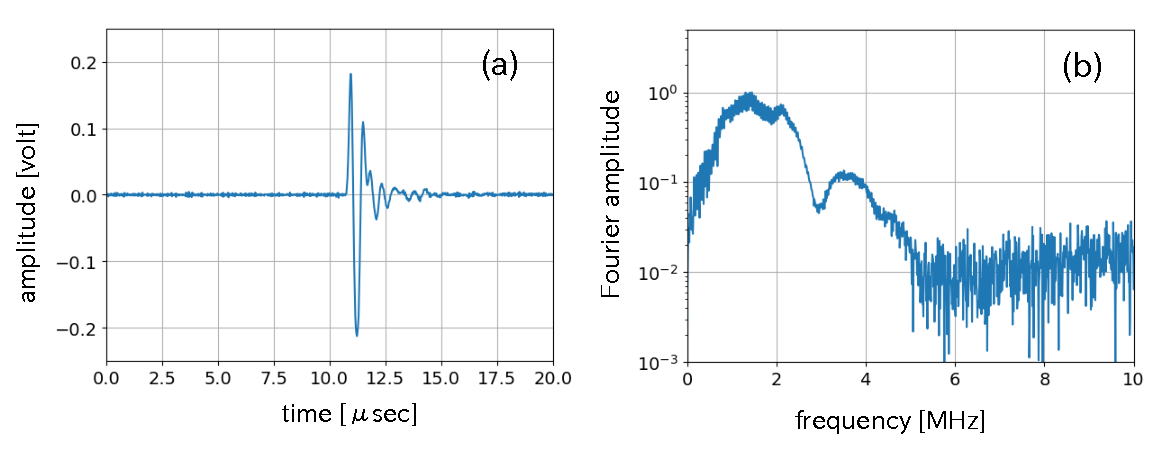
\includegraphics[width=0.9\linewidth]{Figs/fig5.eps} 
	\end{center}
	\caption{
		レーザードップラー振動計で計測した,ラインフォーカス探触子シュー先端部の振動速度波形.
	} 
	\label{fig:fig5}
\end{figure}
%--------------------
\subsection{透過波波形}
花崗岩コア供試体を用いて計測した透過波の計測結果を図\ref{fig:fig5_2}と\ref{fig:fig5_3}に示す。
これらの図には、それぞれ、入射方向の異なる6つの走時プロットが示されている。
各々の走時プロットの横軸は時間$t$($\mu$sec)を、縦軸は計測位置の$y$座標(mm)を表し,
$(t,y)$で観測された波形の振幅をカラー表示したものである。
なお、波形振幅は、最大値で無次元化している。
いずれの入射方向でも、19$\mu$sec前後に大きな振幅を持つ位相の揃った表面波が到達し、その後、
多重散乱に起因するコーダ波が、少なくとも20$\mu$sec程度継続して観測されている。
位相の揃った初動成分の振幅は場所によって大きな変動があり、波形も位置や入射方向によって異なることが分かる。
このことから、個々の観測波形のピーク位置や到達時間から、伝播速度を正確に求めることは困難と言える。
そこで以下では、群遅延から求めた群速度と、
相互相関関数によって評価した遅延時間から求めた音速を用いて、
供試体の音響異方性について調べる。
なお、
%--------------------
\begin{figure}[h]
	\begin{center}
	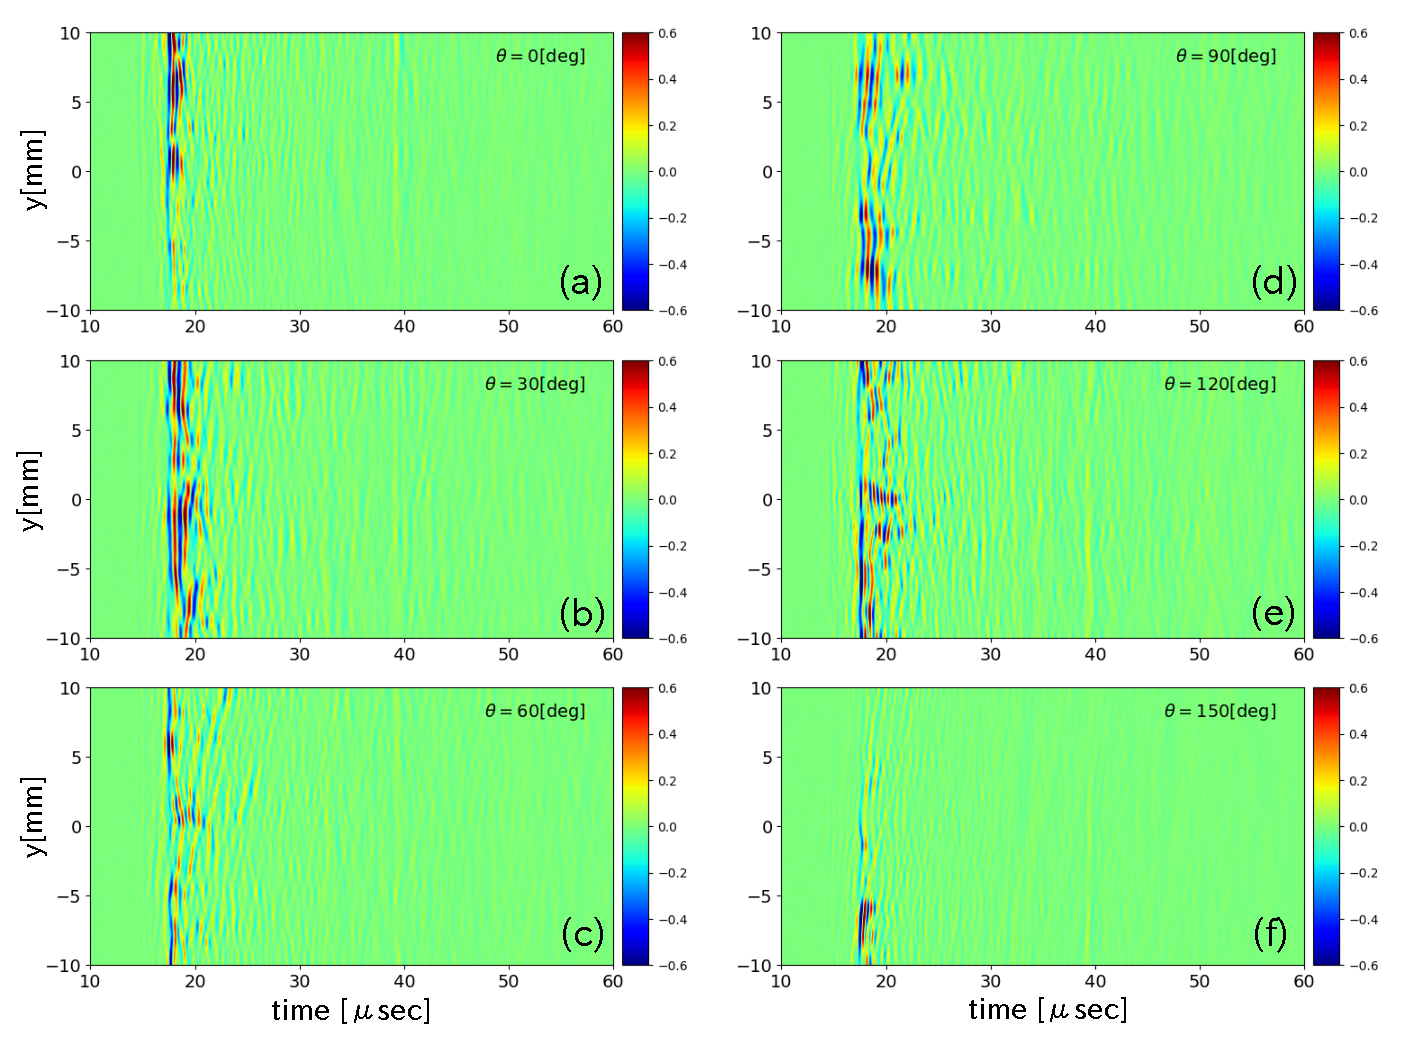
\includegraphics[width=1.0\linewidth]{Figs/fig5_2.eps} 
	\end{center}
	\caption{
		透過波波形の走時プロット(入射方向$\theta=0\sim 150^{\circ}$)
	} 
	\label{fig:fig5_2}が
\end{figure}
%--------------------
\begin{figure}[h]
	\begin{center}
	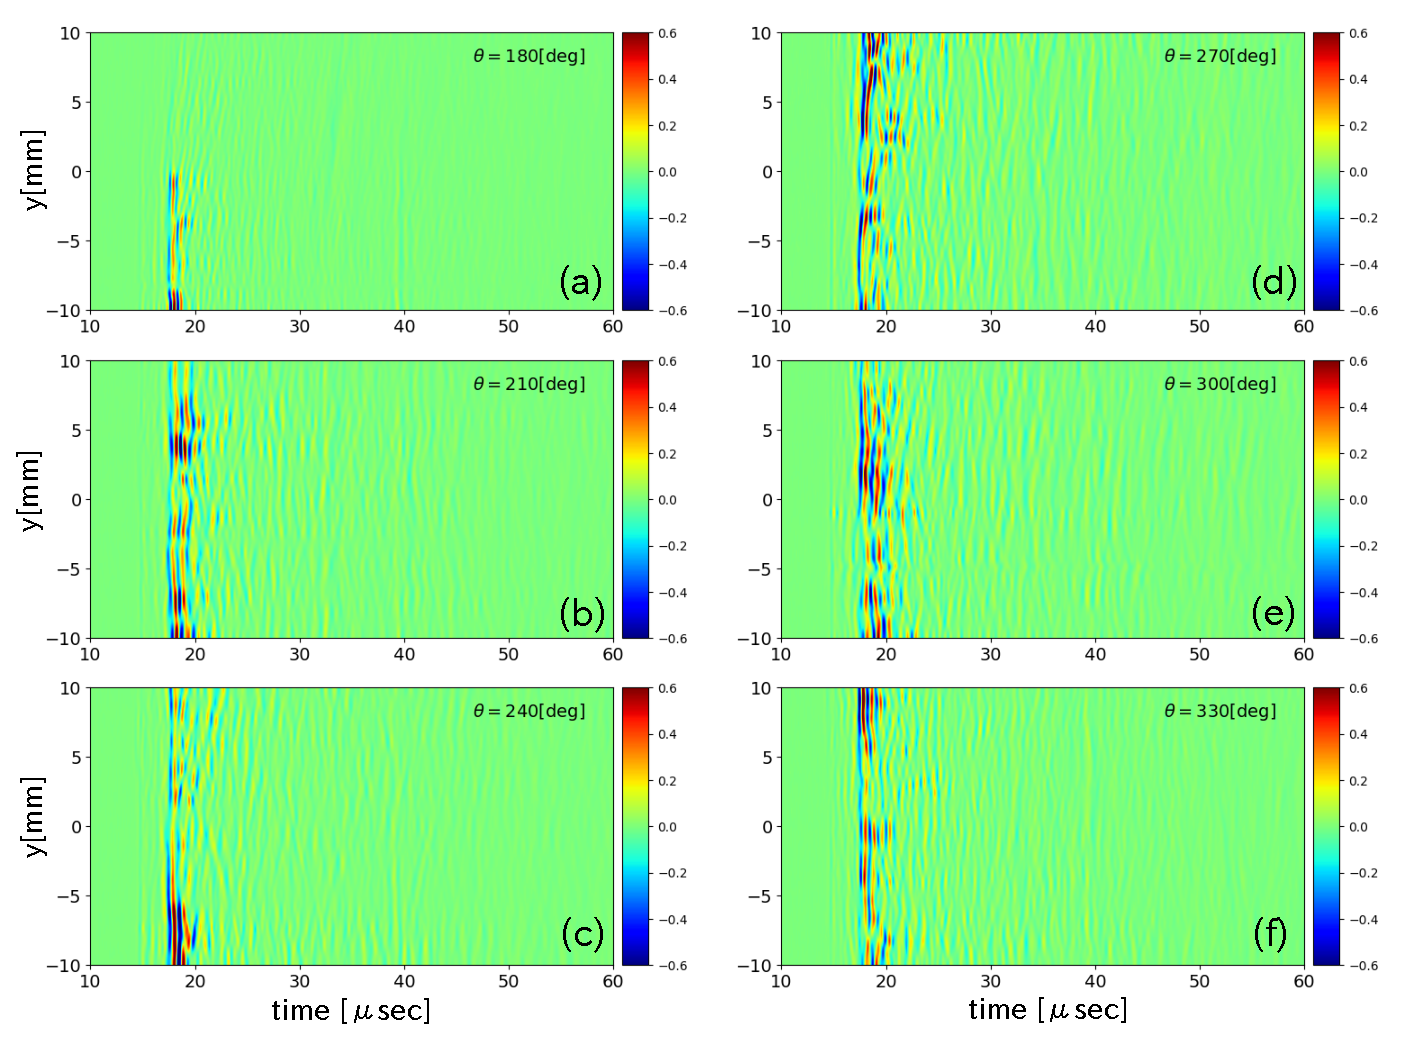
\includegraphics[width=1.0\linewidth]{Figs/fig5_3.eps} 
	\end{center}
	\caption{
		透過波波形の走時プロット(入射方向$\theta=180\sim 330^{\circ}$)
	} 
	\label{fig:fig5_3}
\end{figure}
\subsection{伝播速度の評価}
位相の揃った初動成分を対象として伝播速度の評価を行う。
そのため、時間波形上で窓関数を作用させて初動部分を取り出す。
その際、ここではButterworth関数を用いる。
\begin{equation}
	W(t;t_{1/2},m)=
	\left\{
		1+\left(\frac{t}{t_{1/2}}\right)^m
	\right\}^{-1}
\end{equation}
\begin{equation}
	a(y,t)=a_{mes}(y,t)W(t-t_b;t_{1/2},m)
\end{equation}
ただし、$t_b=18.2$[$\mu$sec], $t_{1/2}=2$[$\mu$sec]で$m=6$.
個々の波形は伝播経路やその周辺の鉱物流の影響を受けて変動する。
何らかの平均値を求める必要がある。
空間的な平均波形を
\begin{equation}
	\left< a\right>(t)=
	\frac{1}{\left| {\cal R}\right|}\int_{\cal R}a(y,t)dy
	\label{eqn:def_mean_wv}
\end{equation}
で定義し、この平均波形から速度を求める。
同時に、個々の計測波形$a(y,t)$から求めた速度の平均値の入射方向依存性を見る。
速度は、群遅延から評価した速度を$c_g$,相互相関から評価した速度を$c_{cor}$と表す。
また、平均波形から評価した速度を$\bar c$, 速度の平均値を$\left< c_{cor}\right>$と表す。
波形$a(t)$のフーリエ変換を
\begin{equation}
	A(\omega)=\int a(t)e^{-i\omega t}dt=\left| A(\omega) \right|e^{i\phi}
	\label{eqn:def_FFT}
\end{equation}
\begin{equation}
	t_g=-\frac{d\phi}{d\omega}
	\label{eqn:}
\end{equation}
\begin{equation}
	c_g=\frac{L}{t_g-t_g^{ref}}
	\label{eqn:def_cg}
\end{equation}
$\bar{c}_g$は、式(\ref{eqn:def_FFT})において$a(t)=<a(y,t)>$としたときに式(\ref{eqn:def_tg})
と式(\ref{eqn:def_cg})から得られる群速度を意味する.
%--------------------
\begin{figure}[h]
	\begin{center}
	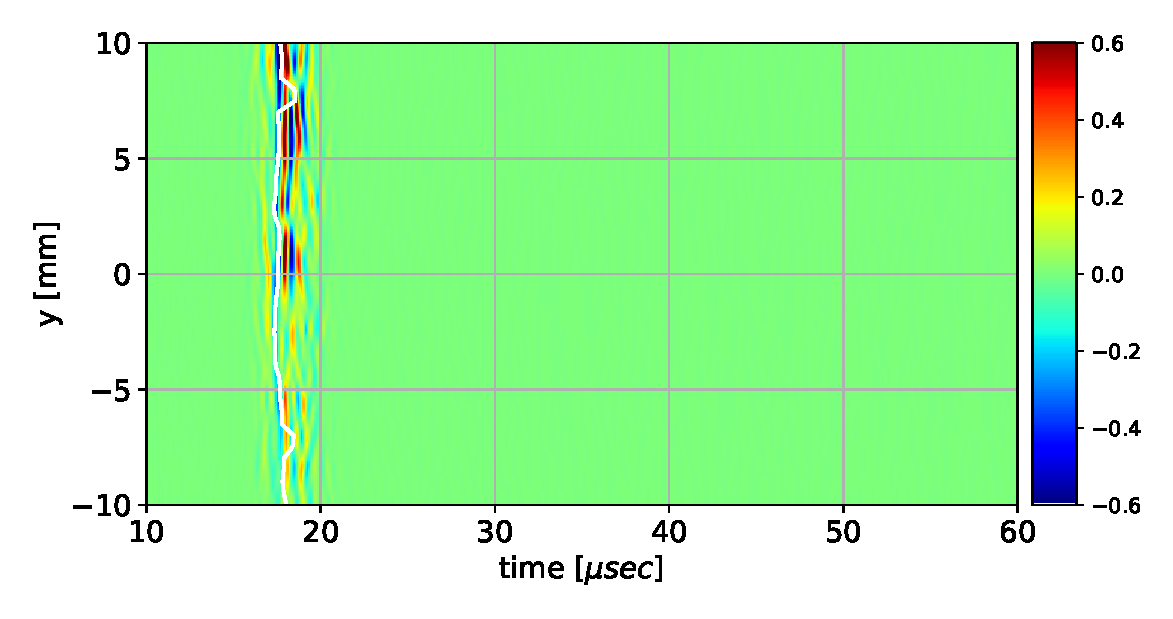
\includegraphics[width=0.7\linewidth]{Figs/fig6.eps} 
	\end{center}
	\caption{
		計測波形の走時プロット(入方向$\theta=0^{\circ}$)
	} 
	\label{fig:fig6}
\end{figure}
%--------------------
\begin{figure}[h]
	\begin{center}
	\includegraphics[width=0.7\linewidth]{Figs/fig7.eps} 
	\end{center}
	\caption{
		計測波形の周波数スペクトログラム(入方向$\theta=0^{\circ}$)
	} 
	\label{fig:fig7}
\end{figure}
%--------------------
\begin{figure}[h]
	\begin{center}
	\includegraphics[width=0.6\linewidth]{Figs/fig8.eps} 
	\end{center}
	\caption{
		平均波形の時刻歴(入射方向$\theta=0^{\circ}$の場合).
	} 
	\label{fig:fig8}
\end{figure}
%--------------------
\begin{figure}[h]
	\begin{center}
	\includegraphics[width=0.6\linewidth]{Figs/fig9.eps} 
	\end{center}
	\caption{
		平均波形の周波数スペクトル(入射方向$\theta=0^{\circ}の場合$).
	} 
	\label{fig:fig9}
\end{figure}
%--------------------
\begin{figure}[h]
	\begin{center}
	\includegraphics[width=0.7\linewidth]{Figs/fig10.eps} 
	\end{center}
	\caption{
		平均波形の位相スペクトル(入射方向$\theta=0^{\circ}$の場合).
	} 
	\label{fig:fig10}
\end{figure}
%--------------------

\section{音響異方性の評価}
各入射方向における測線で得られた波形データから群速度$\left<c_g\right>,\bar c_g$と
相互相関速度$\left<c_{cor}\right>, \bar c_{cor}$を計算した.その結果を
図\ref{fig:fig12}に示す.
この図は横軸が入射方向を,縦軸が音速値(km/s)を示している.
音速値は,概ね2.7(km/sec)から3.15(km/sec)の範囲にあり,主として表面波からなる
波動が観測されていることが分かる.この中で,最も方向による変化が大きいのは
平均群速度$\left<c_g\right>$で,$\theta=150$度と330度の方向で極大,
$\theta=30,240$度の方向で極小となっており,明確に音響異方性を示している.
一方,平均波形$\left<a \right>(t)$から求めた群速度$\bar c_g$の伝播方向による変動は
0.1(km/sec)と小さく,波形の平均化により速度の異方性が弱められることがわかる.
また,相互相関速度$\left<c_{cor}\right>$と$\bar{c}_{cor}$の挙動は,$\bar c_g$の挙動と
よく似ている.相互相関関数の計算では,参照波形として用いた入射波波形と類似した波形部分から到達時間を検出する.
そのため,最もよく位相が揃った波動が到達する時刻が得られるものの,観測点毎の速度変動が反映されにくいと考えられる.
以上のことから,音響異方性の評価には,局所的な群速度の平均$\left<c_g\right>$を見ることが
よいと言える.
%--------------------
\begin{figure}[h]
	\begin{center}
	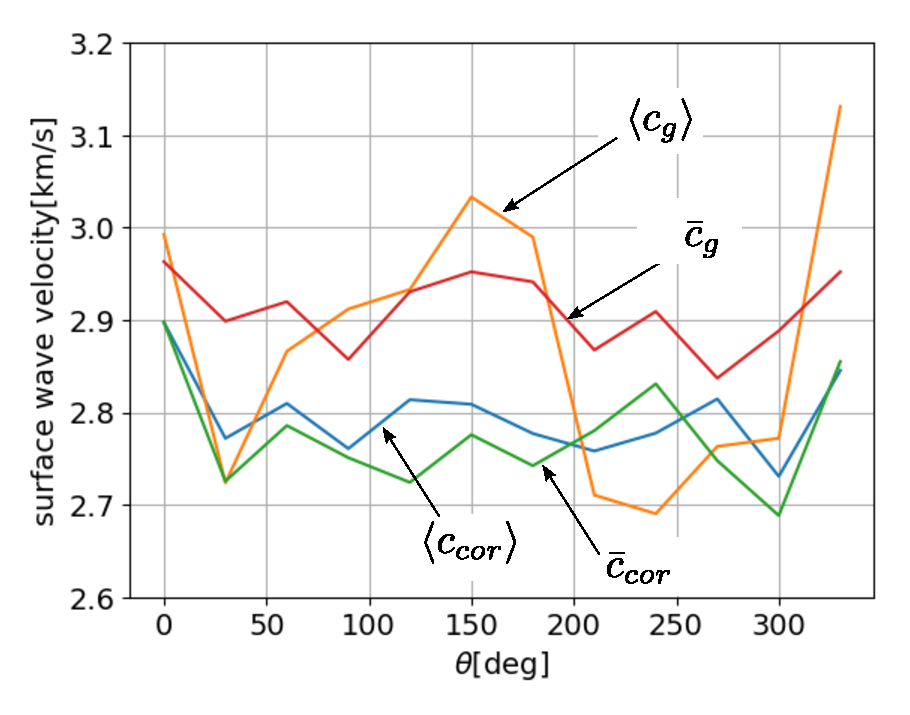
\includegraphics[width=0.8\linewidth]{Figs/fig12.eps} 
	\end{center}
	\caption{
		入射方向による群速度と相互相関速度の変化.
	} 
	\label{fig:fig12}
\end{figure}
%--------------------

ここで,入射方向毎に得られた平均波形$\left<a\right>(t)$を一覧すると,
図\ref{fig:fig11_1}のようになっている.
これら時刻歴波形の振幅はLDV出力の電圧値(mV)を表し,大小関係を波形相互に
比較でき,平均波形の最大振幅は明らかに方向によって変化している.そこで,
平均波形の最大振幅max$\left\{ \left< a \right>\right\}$と,
最大振幅の平均$\left< {\rm max}\left\{ a \right\} \right>$
が入射方向によってどのように変化するかを調べると,
図\ref{fig:fig14}のようになる.
この結果を図\ref{fig:fig12}と比べると,最大振幅の平均
$\left<{\rm max}\left\{a\right\}\right>$
は,$\left<c_g\right>$を上下に反転させたような形となり,強い異方性を
示すことが分かる.これは,群速度の速い方向で振幅が小さく,
遅い方向で振幅が大きくなることを意味する.群速度と振幅値がこのような
相関を示すことは,岩石供試体の見かけの剛性が30度と240度方向で小さく,
150度と0度方向で大きくなるためと考えれば矛盾がない.
なお,平均波形の最大振幅max$\left\{\left<a\right>\right\}$は
最大振幅の平均よりも変動が若干小さい.これは,
波動到達時間の変動を考慮せずに最大値の平均をとる方が,
音響異方性をより敏感に反映した結果が得られることを意味する.
%--------------------
\begin{figure}[h]
	\begin{center}
	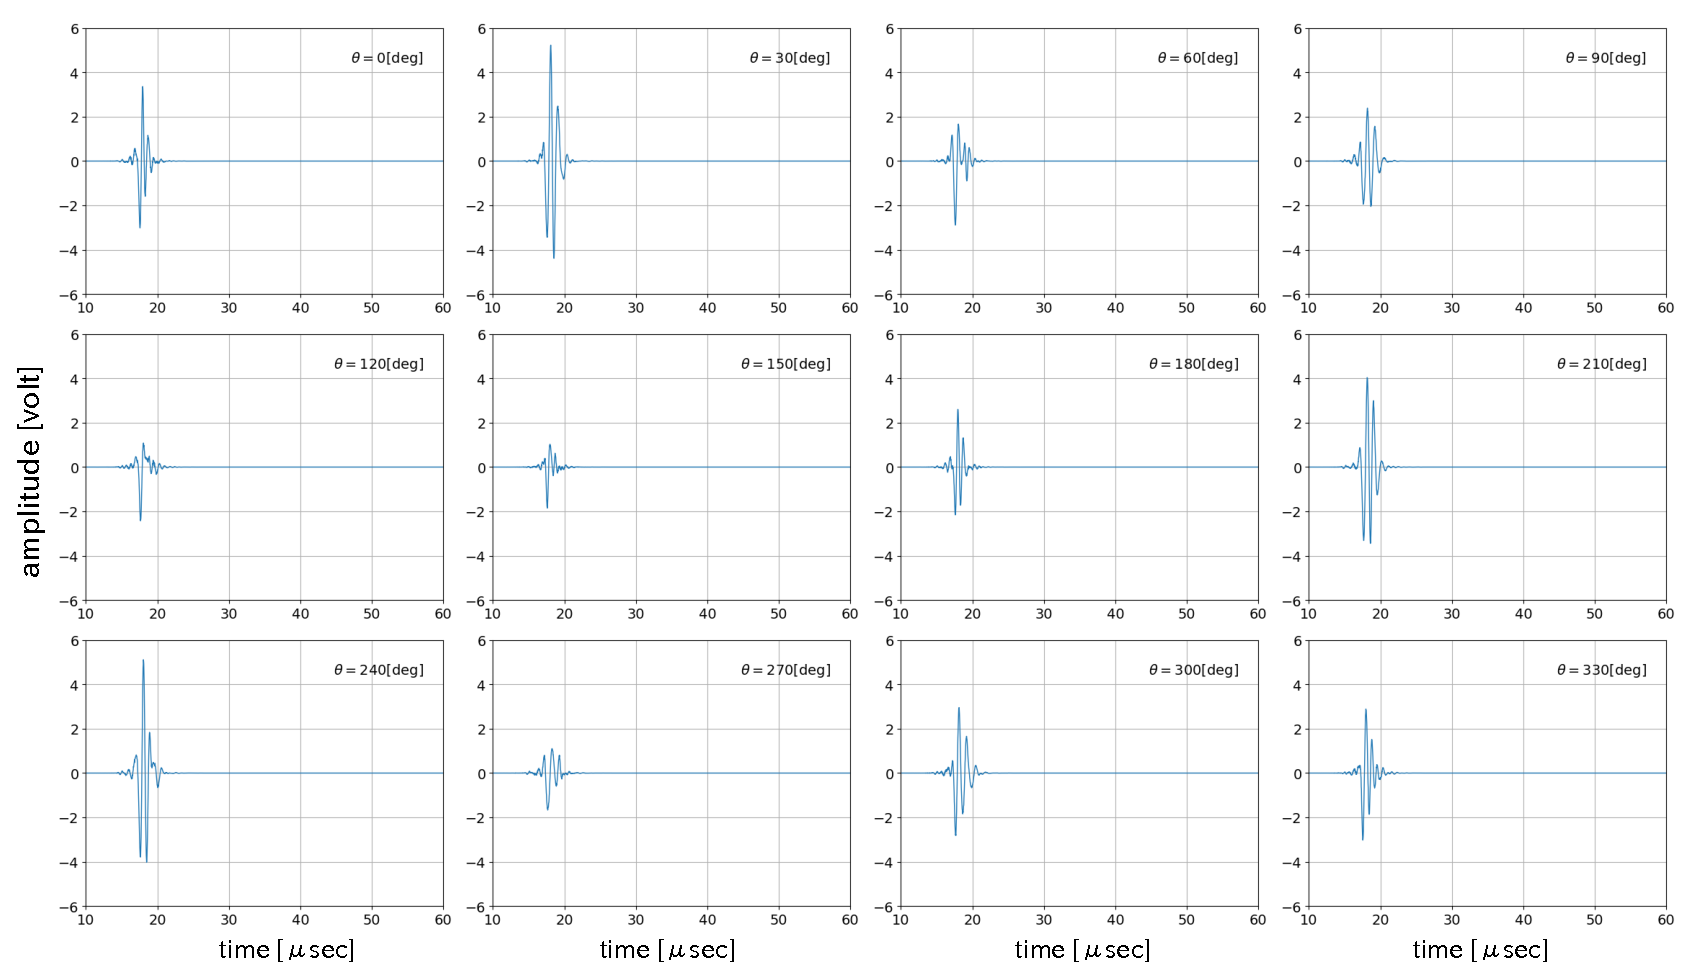
\includegraphics[width=1.0\linewidth]{Figs/fig11_1.eps} 
	\end{center}
	\caption{
		入射方向毎に得られた平均波形の時刻歴.
	} 
	\label{fig:fig11_1}
\end{figure}
%--------------------
\begin{figure}[h]
	\begin{center}
	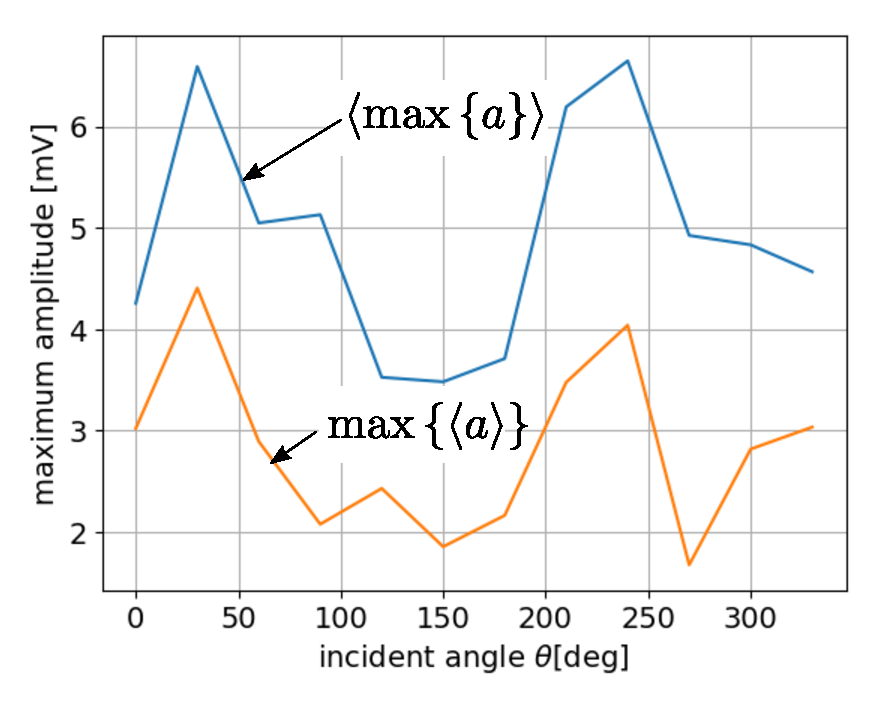
\includegraphics[width=0.8\linewidth]{Figs/fig14.eps} 
	\end{center}
	\caption{
		入射方向による最大振幅値の変化.
	} 
	\label{fig:fig14}
\end{figure}
最後に,平均波形の周波数スペクトル
\begin{equation}
	\left< A \right> (\omega) = \int \left<a\right>(t)e^{-i\omega t}dt
	\label{eqn:ave_A}
\end{equation}
を,入射方向毎に計算した結果を図\ref{fig:fig11_2}に示す.
これらの結果を見ると,周波数帯域はいずれの方向でも3MHz程度までとなっており,
その点に大きな違いは無い.一方,ピーク周波数には明らかなばらつきがあることに
気付く.そこで,平均波形のピーク周波数argmax$\left< A \right>$と,
個々の観測波形に対するピーク周波数の平均$\left< {\rm argmax }\left\{ A \right\}\right>$を求め,
角度との関係を示せば,図\ref{fig:fig13}のようになる.この図より,
ピーク周波数の平均$\left< {\rm argmax }\left\{ A \right\}\right>$は
$\left< c_g\right>$と似た傾向を示すことが分かる.具体的には,
群速度平均が大きな方向ではピーク周波数平均が高く,群速度平均が小さな方向では,
ピーク周波数平均は低くなっている.
これは,見かけの剛性が高い方が高周波の波を伝えやすく,みかけの剛性が低い方が
高周波成分を伝えにくいことを意味する.ここで,見かけの剛性と周波数が相関することは,
剛性の変化がマイクロクラックに起因したものであることを意味する.
なぜなら,線形弾性体では剛性の大小は振幅や音速に影響するが,周波数応答には
関与せず,剛性の周波数依存性は,界面の接触や滑りによってのみ生じるためである.
従って,ここで示した音響異方性に関する結果は,弾性波を使ったき裂評価において有用な
情報であると考えることができる.
なお,ピーク周波数の平均が,平均波形のピーク周波数よりも変動が小さい理由は
平均最大振幅と平均波形の最大振幅の大小に関する理由と同様である.
%--------------------
\begin{figure}[h]
	\begin{center}
	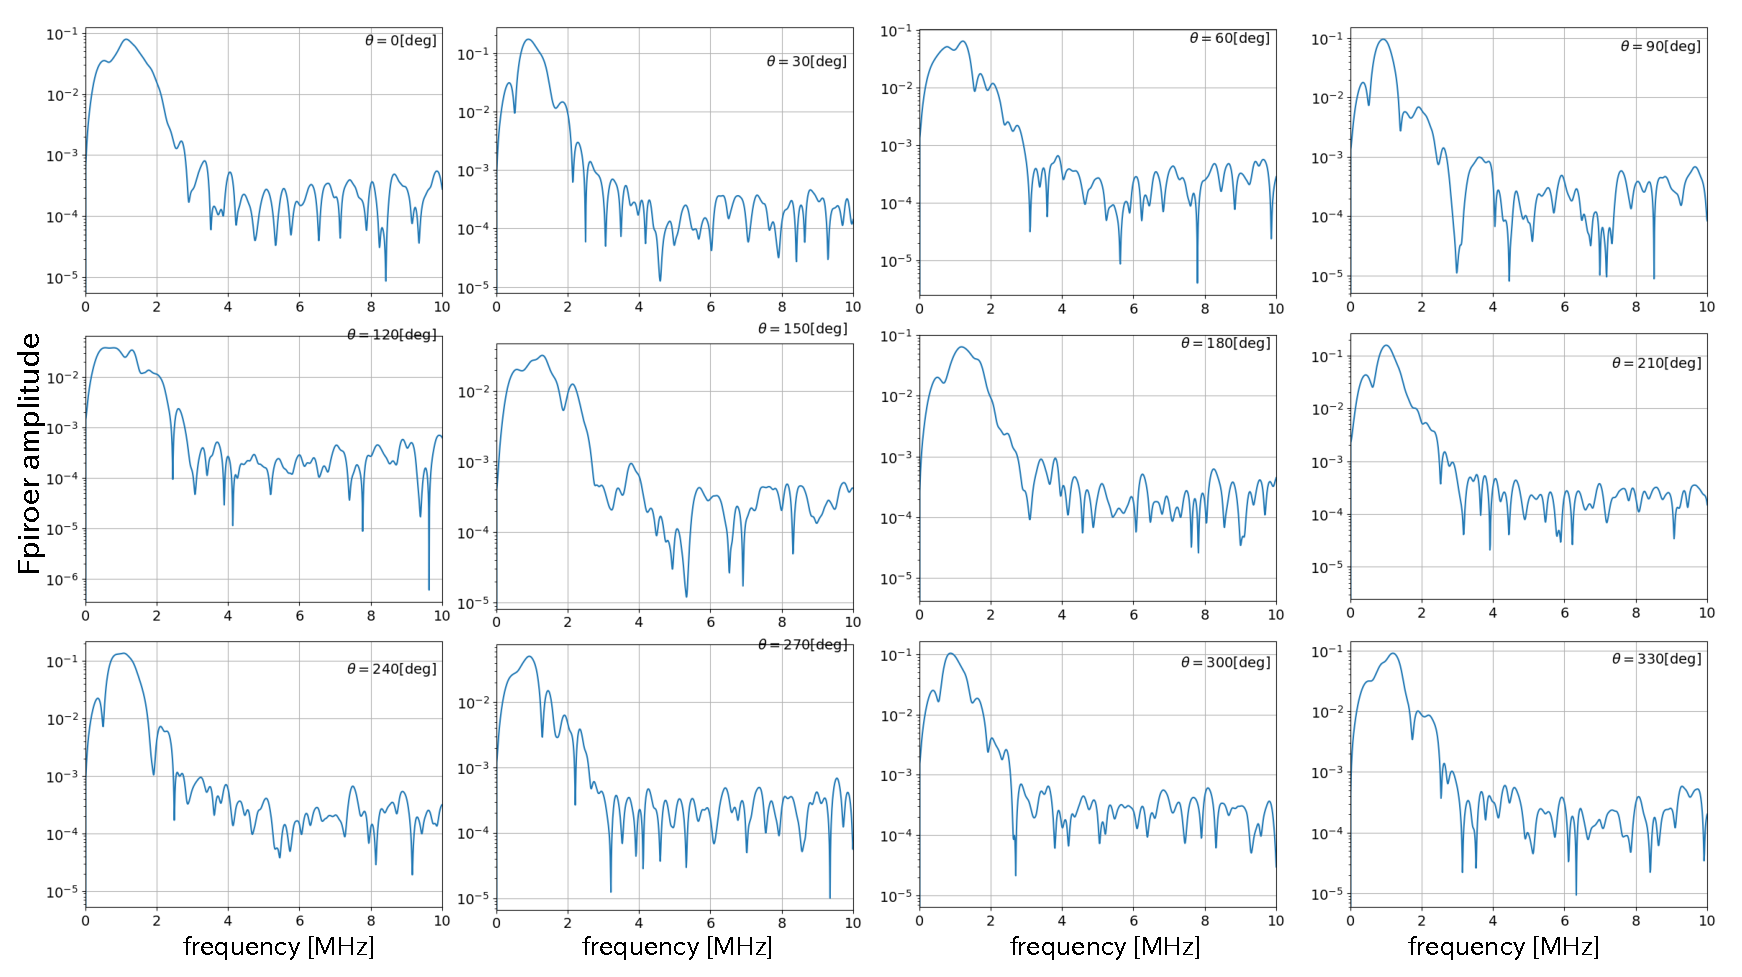
\includegraphics[width=1.0\linewidth]{Figs/fig11_2.eps} 
	\end{center}
	\caption{
		入射方向毎に得られた平均波形の周波数スペクトル.
	} 
	\label{fig:fig11_2}
\end{figure}
\begin{figure}[h]
	\begin{center}
	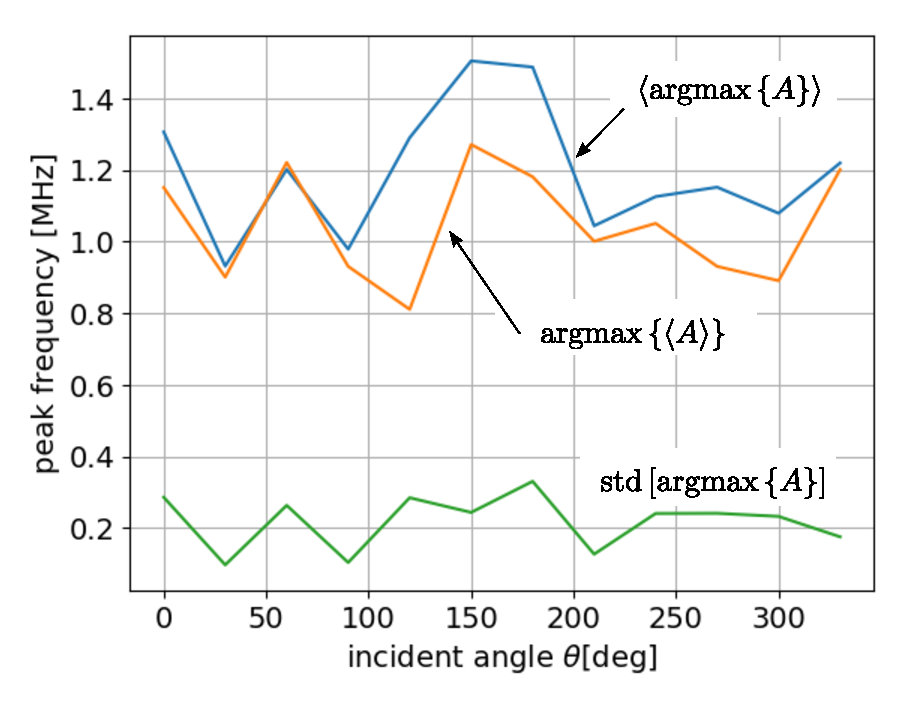
\includegraphics[width=0.8\linewidth]{Figs/fig13.eps} 
	\end{center}
	\caption{
		入射方向によるピーク周波の変化.
	} 
	\label{fig:fig13}
\end{figure}
%--------------------


%--------------------
\newpage
\section{まとめ}
 本研究では,計測した表面波の波形データを使い,花崗岩供試体の音響異方性について
調べた.音響異方性を調べるためには,弾性波伝播挙動の方向による変化を調べる
ことが必要であるため,ここでは,表面波の励起を供試体表面に取り付けた圧電センサーで行い,
圧電センサーの向きを変化させ,入射方向を様々に変えた場合の表面波データを取得した.
その際,十分な信号強度を得るため,超音波の送信には特別に設計および作成した
ラインフォーカス探触子を用いいた.この探触子は,曲率をつけた圧電素子で発生させた
縦波をポリエーテルイミドで作成したくさび状のシュー先端部に集束させることで,
岩石供試体中に強い超音波を入射する.その結果として,従来の探触子よりも20倍程度
強度で超音波を送信することが可能となった.ラインフォーカス探触子は,
擬似的な線音源を作り出し,試料内部に減衰の影響を受けにくい平面波を励起することが
可能で,これまで難しかった2から3MHz程度まで帯域を持つ超音波の送受信を実現する
ことができた.

以上の方法で励起した表面波を,レーザードップラー振動計で観測し,
伝播方向を様々に変えて表面波の速伝播挙動を調べた.
一連の計測結果を処理し,群速度,相互相関速度,最大振幅とピーク周波数について
伝播方向の関係を調べたところ,実験に用いた花崗岩供試体は,概ね直交異方性を示す
ことをが明らかとなった.特に,群速度と最大振幅およびピーク周波数には,互いに
相関が認められることが示され,これは,き裂の存在に起因した見かけの剛性変化が
原因であると解釈すれば必然的な結果であること言える.
また,計測結果から合成した平均波形よりも,個々の波形から音速や振幅値を評価し,
その平均をとる方が,供試体の音響異方性をより感度良く捉えることができる
ことも明らかとなった.そのためには,従来の圧電センサーによる受信でなく,
本研究のようにLDVによる詳細な計測が必要となる.

以上のような知見は,今後,花崗岩における弾性波伝播モデルを構築し,
その妥当性を検証する上で有用な知見になると考えられる.
また,今後,音響異方性や弾性波伝播挙動の信頼できるモデルを構築することができれば,
超音波計測で評価した音響異方性から,き裂密度や配向性を非破壊的に推定することも
可能と刷ることが期待できる.そのような技術の開発に向け,今後は,超音波計測結果を
再現するための弾性波伝播モデルの構築に取り組む必要がある.
また,送受信する超音波の周波数帯域を変化させることで,
音響異方性評価における空間解像度を調整できるようにすることも重要な技術的課題
と考えられる.更に,現場計測への適用や実用化の面では,検査効率の向上も
重要であり,そのためには超音波の受信だけでなく送信についても非接触で行う
方法を確立することも必要と考えられる.
\section{付録(全計測波形とその周波数スペクトル)}
本付録では、計測波形とその周波数スペクトルを図\ref{fig:fig15}-\ref{fig:fig18}に
測線毎に計算した平均波形とその周波数スペクトルを図\ref{fig:fig19}-\ref{fig:fig20}
に示す。これらは、計測したままの波形(Butterworth窓関数を作用させる以前の状態)を示した
もので、本文中に示した結果と本節の結果を比較すれば、窓関数を作用させることによって
初動部分の波形や周波数スペクトルの構造が、ほとんど変化していないことを確認することができる。
%--------------------
\begin{figure}[h]
	\begin{center}
	\includegraphics[width=1.0\linewidth]{Figs/fig15.eps} 
	\end{center}
	\caption{
		計測波形の走時プロット($\theta=0\sim 150^{\circ}$).
	} 
	\label{fig:fig15}
\end{figure}
%--------------------
\begin{figure}[h]
	\begin{center}
	\includegraphics[width=1.0\linewidth]{Figs/fig16.eps} 
	\end{center}
	\caption{
		計測波形の走時プロット($\theta=180\sim 330^{\circ}$).
	} 
	\label{fig:fig16}
\end{figure}
%--------------------
\begin{figure}[h]
	\begin{center}
	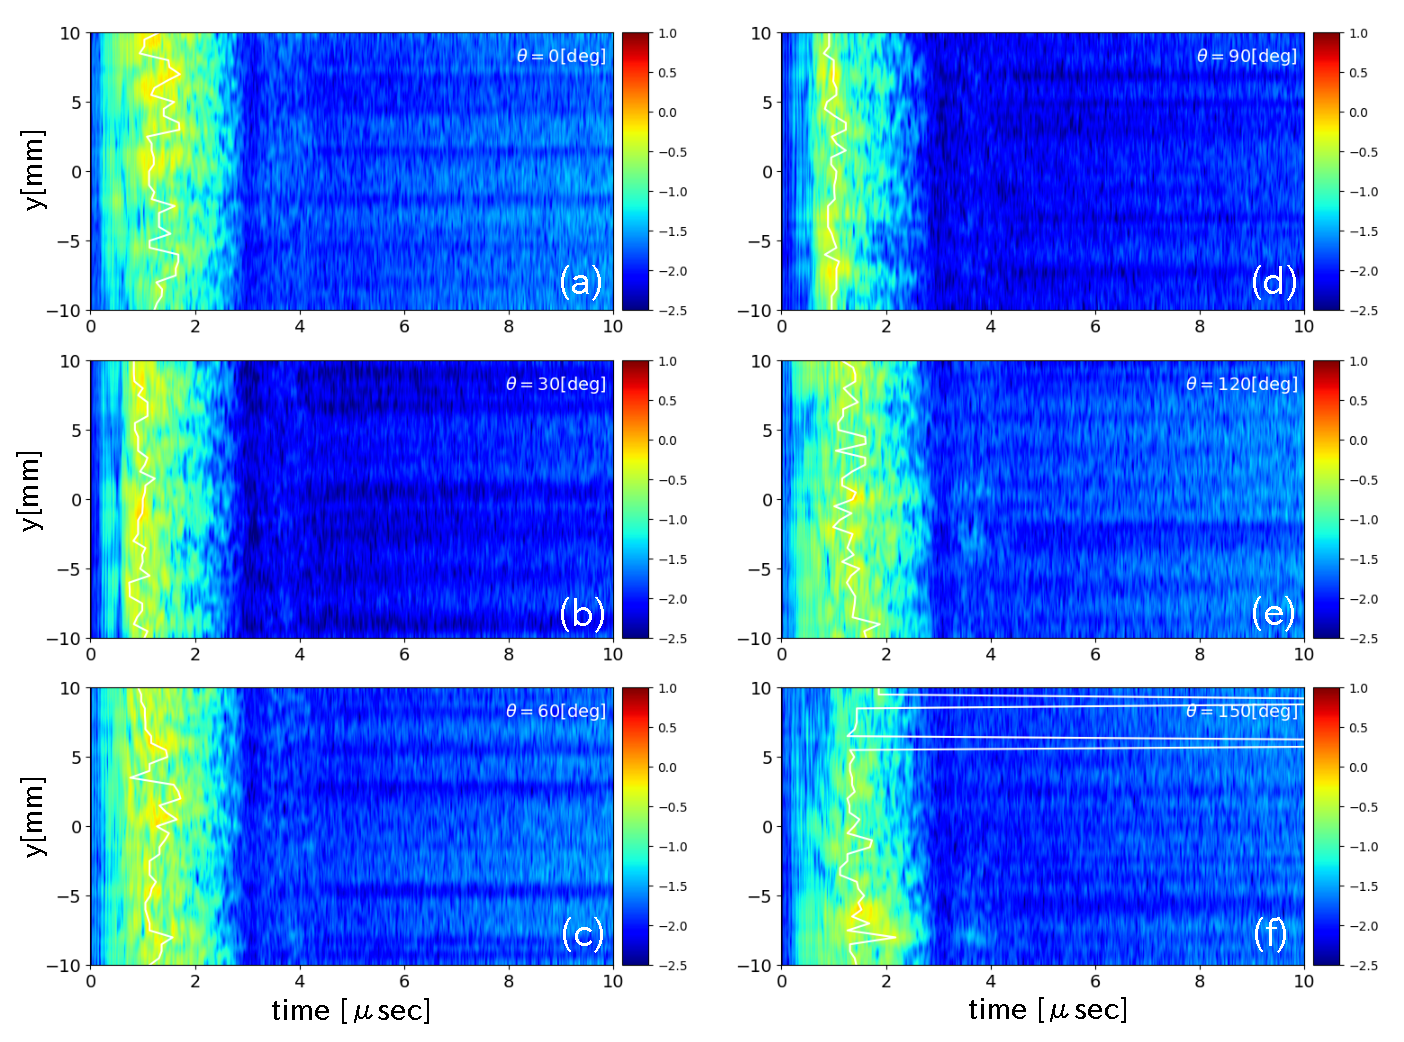
\includegraphics[width=1.0\linewidth]{Figs/fig17.eps} 
	\end{center}
	\caption{
		対数スケールで示した計測波形の周波数スペクトル($\theta=0\sim 150^{\circ}$).
	} 
	\label{fig:fig17}
\end{figure}
%--------------------
\begin{figure}[h]
	\begin{center}
	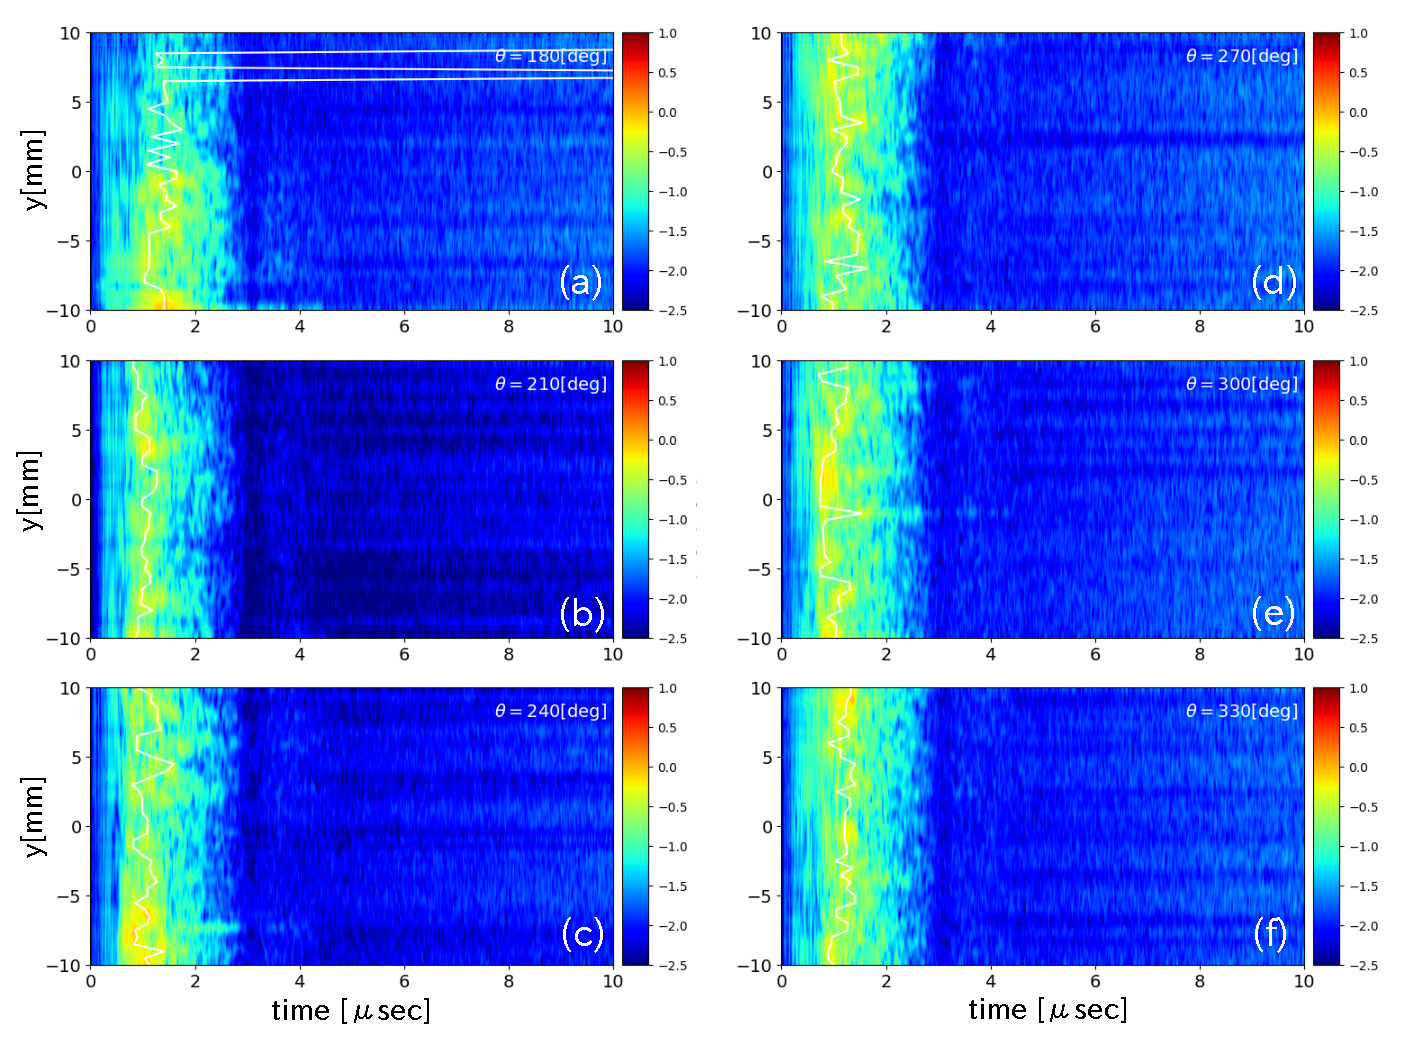
\includegraphics[width=1.0\linewidth]{Figs/fig18.eps} 
	\end{center}
	\caption{
		対数スケールで示した計測波形の周波数スペクトル($\theta=180\sim 330^{\circ}$).
	} 
	\label{fig:fig18}
\end{figure}
%--------------------
\begin{figure}[h]
	\begin{center}
	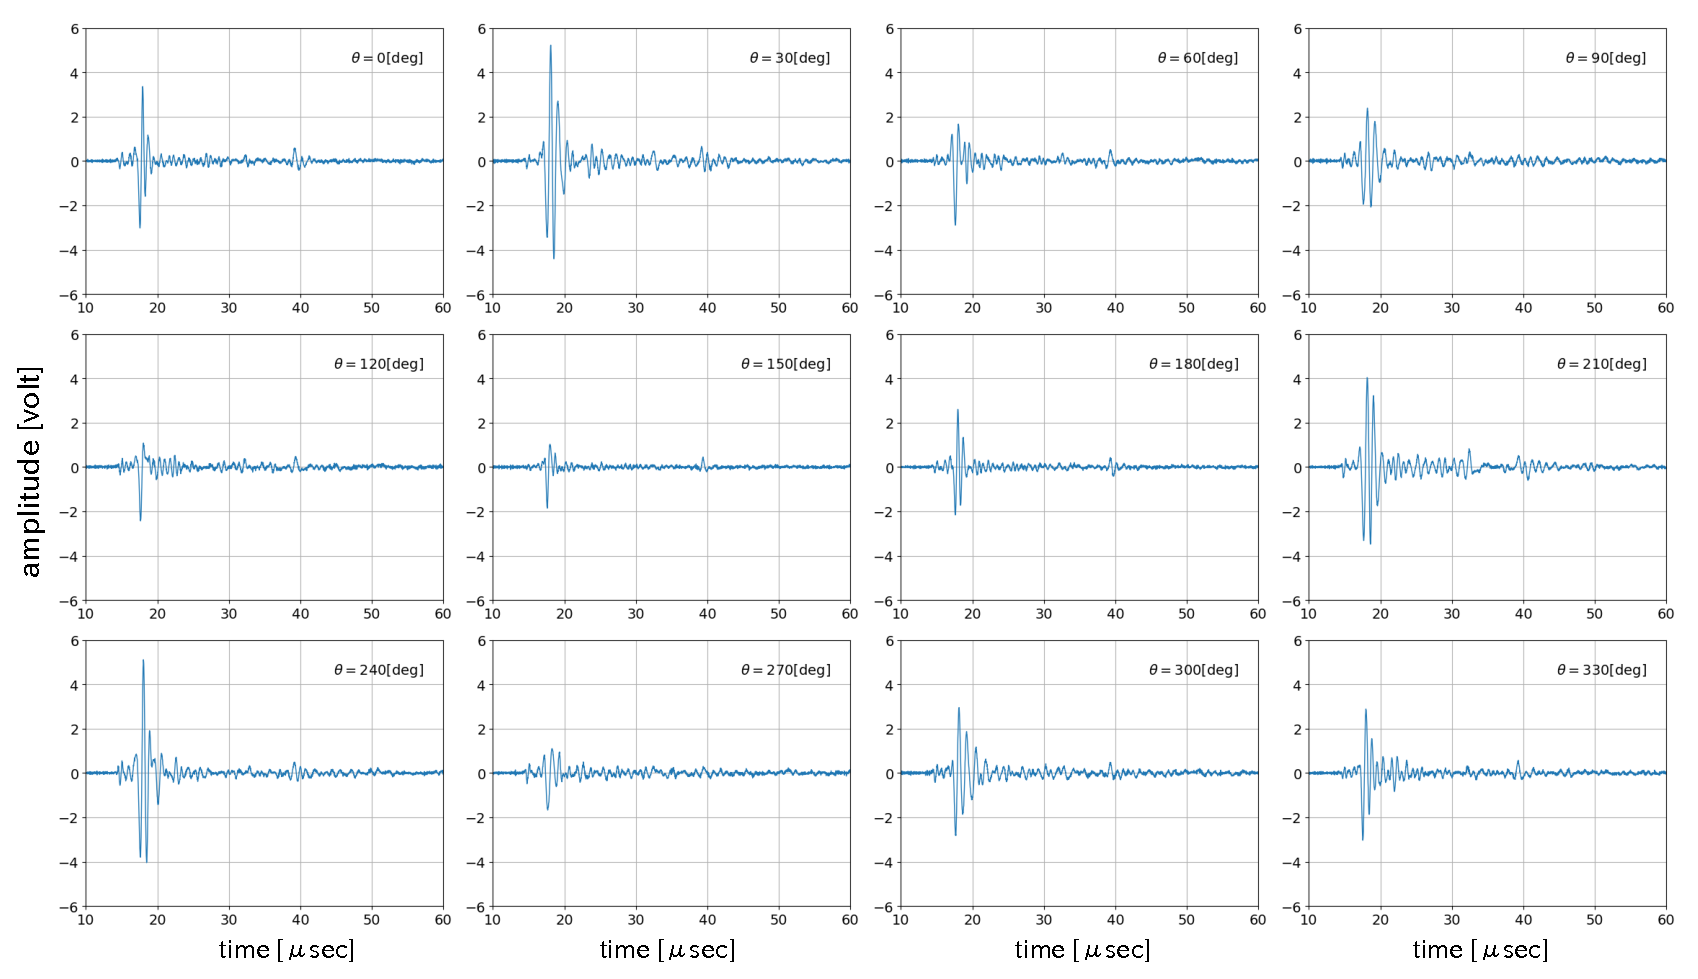
\includegraphics[width=1.0\linewidth]{Figs/fig19.eps} 
	\end{center}
	\caption{
		測線毎に算出した平均波形.
	} 
	\label{fig:fig19}
\end{figure}
%--------------------
\begin{figure}[h]
	\begin{center}
	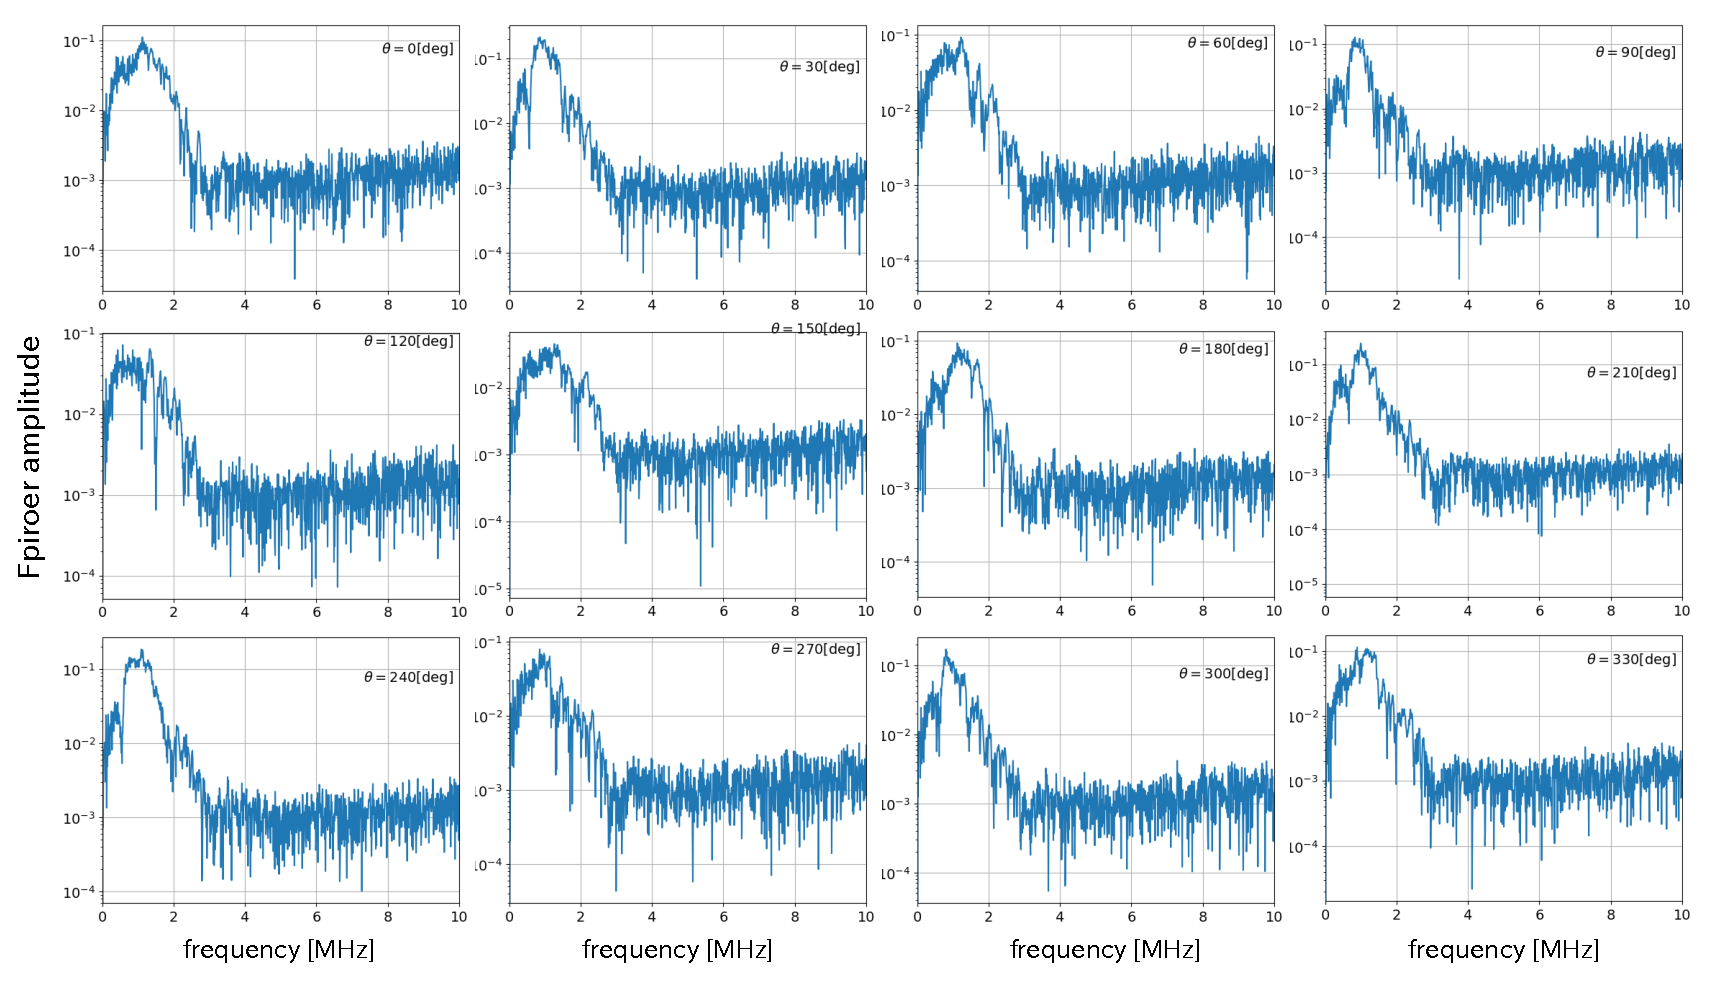
\includegraphics[width=1.0\linewidth]{Figs/fig20.eps} 
	\end{center}
	\caption{
		測線毎に算出した平均波形の周波数スペクトル.
	} 
	\label{fig:fig20}
\end{figure}
%--------------------

\end{document}
